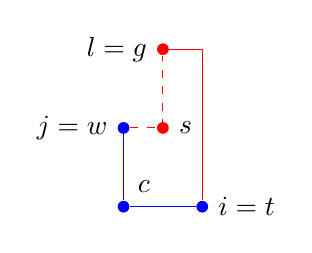
\begin{tikzpicture}

    % Blue points forming an L-shape
    \node[fill=blue, circle, inner sep=1.5pt, label=above right:\(\boldvec{c}\)] (c) at (0, 0) {};
    \node[fill=blue, circle, inner sep=1.5pt, label=right:{\(\boldvec{i} = \boldvec{t}\)}] (i) at (1, 0) {};
    \node[fill=blue, circle, inner sep=1.5pt, label=left:{\(\boldvec{j}= \boldvec{w}\)}] (j) at (0, 1) {};
    
    % Draw lines to form the L-shape
    \draw[blue] (c) -- (i);
    \draw[blue] (c) -- (j);
    
    % Red point near the L-shape
    \node[fill=red, circle, inner sep=1.5pt, label=left:{\(\boldvec{l} = \boldvec{g}\)}] (l) at (0.5, 2) {};
    \node[fill=red, circle, inner sep=1.5pt, label=right:{\( \boldvec{s}\)}] (s) at (0.5, 1) {};

    % Connect the red point to the blue L-shape with another L-shape
    \draw[red] (l) -- (1,2) -- (i) ;
    \draw[red, dashed] (j) -- (0.5, 1) -- (l) ;
    
\end{tikzpicture}